\documentclass[11pt]{article}
\usepackage[margin=1in]{geometry}
\usepackage{amsmath,amssymb,amsthm,booktabs,tikz}
\usepackage[hidelinks]{hyperref}
\hypersetup{pdftitle={Crossing rates for coherent Bell pairings and packed loops},pdfauthor={zhangjinba}}
\newtheorem{theorem}{Theorem}
\newtheorem{proposition}[theorem]{Proposition}
\newcommand{\C}{\mathbb C}
\newcommand{\rate}{\mathcal R}
\newcommand{\tr}{\operatorname{Tr}}
\title{Crossing rates for coherent Bell pairings\\and packed loops}
\author{zhangjinba}
\date{November 25, 2026}
\begin{document}
\maketitle
\begin{abstract}
Four parties on a square share a coherent sum of the two ways to pair adjacent
parties by maximally entangled states of local dimension \(q\). How many pairs
on both diagonals can they extract by local linear maps on many copies?
Using the Euclidean prices theorem, we bound the number of output copies per
input copy by \((1+1/\log_2 q)/\sqrt{2}\). For \(q\ge6\) this is strictly
below one, although every bipartite flattening rank and every singleton
quantum functional allows unit rate. A projection and routing protocol gives
a lower bound of \(\tfrac12\log_q\lfloor q/2\rfloor\) for \(q\ge4\).
The same local tensor is a vertex weight of the completely packed loop model.
On square patches we obtain a bound on independent boundary color
transmission in terms of the fraction of vertices with arbitrary weights.
\end{abstract}

\section{A four-party conversion}

Let \(V=\C^q\), \(q\ge2\), and let \(E_{ij}(q)=\sum_{s=1}^q e_s^{(i)}
\otimes e_s^{(j)}\) be an unnormalized Bell pair. Products below group indices
at the same party. Number the corners of a square in cyclic order and set
\begin{align*}
 A_q&=E_{12}(q)E_{34}(q), & B_q&=E_{14}(q)E_{23}(q),\\
 U_q&=A_q+B_q,             & D_q&=E_{13}(q)E_{24}(q).
\end{align*}
Both summands of \(U_q\) occupy the same four copies of \(V\). In particular
each party has exactly \(q\) local coordinates and receives no label
identifying a summand. Figure~\ref{fig:pairings} depicts the three tensors.

\begin{figure}[ht]
\centering
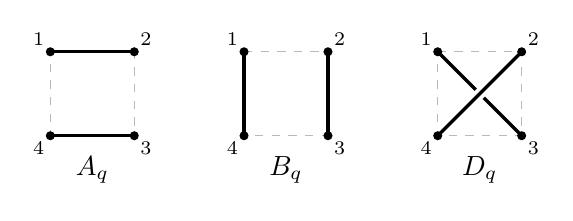
\begin{tikzpicture}[scale=.82]
\foreach \x/\tag in {0/A_q,3/B_q,6/D_q}{
\begin{scope}[xshift=\x cm]
\coordinate (a) at (0,1.3); \coordinate (b) at (1.3,1.3);
\coordinate (c) at (1.3,0); \coordinate (d) at (0,0);
\draw[gray!55,dashed] (a)--(b)--(c)--(d)--cycle;
\ifnum\x=0 \draw[very thick] (a)--(b) (c)--(d); \fi
\ifnum\x=3 \draw[very thick] (a)--(d) (b)--(c); \fi
\ifnum\x=6 \draw[very thick] (a)--(c); \draw[white,line width=4pt] (b)--(d);
\draw[very thick] (b)--(d); \fi
\foreach \p/\pos/\n in {a/above left/1,b/above right/2,c/below right/3,d/below left/4}
{\fill (\p) circle (2pt) node[\pos,inner sep=2pt,font=\scriptsize]{\n};}
\node at (.65,-.53) {$\tag$};
\end{scope}}
\end{tikzpicture}
\caption{Each solid segment shares one independent \(q\)-valued label.
The diagonal segments pass through one another without an extra party.}
\label{fig:pairings}
\end{figure}

Write \(T\succeq S\) if linear maps, one at each party, send \(T\) to a
nonzero multiple of \(S\). Physically this allows a postselected branch of
a local protocol, with no lower bound on its success probability. Define
\[
 \rate_q=\sup\bigl\{m/n: n\ge1,\ m\ge0,\
                     U_q^{\otimes n}\succeq D_q^{\otimes m}\bigr\}.
\]
Any feasible block can be repeated. A map at one party may use all its input
copies jointly. All logarithms without a base below have base two.

\begin{theorem}\label{thm:square}
Assume the Euclidean prices theorem of \cite[Thm.~1.1]{price}.
For every \(q\ge2\),
\[
 \rate_q\le \min\{1,\alpha_q\},\qquad
 \alpha_q=\frac{1+1/\log q}{\sqrt2}.
\]
For \(q\ge4\), one also has
\(\rate_q\ge\tfrac12\log_q\lfloor q/2\rfloor\).
In particular \(1/3\le\rate_8\le4/(3\sqrt2)<1\).
\end{theorem}

The asymptotic restriction order and its quantum functionals are studied
in \cite{cvz,botero}. The geometric input in Theorem~\ref{thm:square}
is the simultaneous pricing of all wires and direct sums at a fixed
placement. The prescribed input \(U_q^{\otimes n}\) fixes every summand
before any maps are chosen. This differs from optimizing a decomposition of
the diagonal tensor over summands of bounded flattening ranks, as in the
sharp common crossing exponent of \cite{price}. Our comparisons below
evaluate all seven individual cuts and the singleton quantum functionals.
Determining the bounds furnished by general higher-order weightings
of \cite{botero} on this pair remains open here.

\section{Cut ranks, singleton entropies and the geometric bound}

For the seven unordered bipartitions, the ranks of the two tensors are
\[
\begin{array}{lccc}
\toprule
\text{Cut} & \text{Multiplicity} & U_q & D_q\\
\midrule
 i\mid\{1,2,3,4\}\setminus\{i\} &4 &q&q\\
 12\mid34,\ 14\mid23 &2&q^2&q^2\\
 13\mid24 &1&q(q+1)/2&1\\
\bottomrule
\end{array}
\]
Indeed, let \(P(x\otimes y)=y\otimes x\) and \(v=\sum_s e_s\otimes e_s\).
The \(12\mid34\) matrix of \(U_q\) is \(P+vv^{\mathsf T}\).
The determinant lemma gives determinant \((1+q)\det P\), since \(Pv=v\).
Reflection gives the second adjacent cut. The opposite cut has matrix
\(I+P\), whose image is \(\operatorname{Sym}^2 V\). Full adjacent rank
forces full singleton rank. For \(D_q\) each wire crossing a cut multiplies
the rank by \(q\). Thus all directional rank inequalities permit \(m=n\),
and in particular imply the upper bound \(m/n\le1\).
At \(m=n\) full local ranks force the four maps to be invertible, whereas the
opposite-cut ranks differ. This excludes exact equality in a finite block.
The directional inequalities still permit \(m=n-1\) for every \(n\).

There is also an entropy comparison. For either normalized tensor and each
individual party the reduced state is \(I/q\): \(O^{\otimes4}\) fixes
every pairing for each real orthogonal matrix \(O\), and a matrix commuting
with all sign changes and permutations is scalar. For a probability
weighting \(\theta\) on the four singletons, the quantum functional of
\cite{cvz} is two raised to the maximum weighted marginal entropy on
the normalized orbit closure. Each entropy is at most \(\log q\); both
given tensors attain that value at every party simultaneously. Thus the
functional is \(q\) on both input and target for every such \(\theta\).

\paragraph{The Euclidean price.}
We use three consequences of \cite[Thm.~1.1 and the calculus of prices]{price}.
On finite sets of planar sites there is a compatible price \(H\) that is
additive on tensor products and monotone under local linear maps.
Inserting a site with a trivial factor preserves the price, so local
contraction of two legs at a common site can only decrease it.
A \(q\)-wire between \(x,y\) has price \(\|x-y\|\log q\).
For two tensors on the same output spaces at a planar set \(S\),
\begin{equation}\label{eq:sum}
 H(T_1+T_2)\le \max\{H(T_1),H(T_2)\}+W(S),
\end{equation}
where \(W(S)\) for a nondegenerate polygon is half the perimeter of its
convex hull. Indeed, the ordinary sum is a local image of the direct sum.
The spectral point \(2^{H/W(S)}\) is additive on that direct sum, giving
\eqref{eq:sum}. A nonzero scalar factor leaves \(H\) unchanged.

\begin{proof}[Proof of Theorem~\ref{thm:square}]
Place the four parties at the corners of a unit square. Then \(W(S)=2\),
both adjacent pairings have price \(2\log q\), and \(D_q\) has price
\(2\sqrt2\log q\). For any feasible \(n,m\), \eqref{eq:sum} gives
\[
 2\sqrt2\,m\log q=mH(D_q)\le nH(U_q)\le n(2\log q+2).
\]
This is strict against unit rate exactly when \(q>2^{1+\sqrt2}\),
or \(q\ge6\) among integers. The fixed-placement closure lemma of
\cite{price} gives the same upper bound if at each block size the target
belongs to the algebraic closure of the local images. This extension
concerns exact algebraic degeneration in each fixed format.

For the lower bound put \(d=\lfloor q/2\rfloor\). Choose two disjoint
sets of \(d\) coordinates. Project sites 1 and 2 to the first set,
and sites 3 and 4 to the second. This kills \(B_q\), leaving two
independent horizontal pairs of rank \(d\). Rotating the projections on a
second input copy leaves two vertical pairs. Four inputs therefore give
two independent rank-\(d\) pairs on every side of the square. Route
the four paths \(123,143,214,234\), using distinct pairs whenever two
paths traverse the same side. Contracting with a Bell covector at the
middle of each path joins its endpoint labels. The first two paths give
two \(13\) pairs and the last two give two \(24\) pairs, yielding
\(D_{d^2}\). Repeating the block \(k\) times and truncating each
diagonal's label space gives \(\lfloor 2k\log_q d\rfloor\) target copies
from \(4k\) inputs. Taking the supremum proves the claim.
\end{proof}

\section{Boundary colors in a completely packed loop model}

Put a cell in each unit square of \([0,L]^2\), with one color in
\(\{1,\ldots,q\}\) on each edge midpoint. In cyclic order \(N,E,S,W\),
a regular cell has Boltzmann weight
\begin{equation}\label{eq:boltz}
 a\,\delta_{i_N,i_E}\delta_{i_S,i_W}
 +b\,\delta_{i_N,i_W}\delta_{i_S,i_E}.
\end{equation}
The positive-weight case takes \(a,b>0\); the bounds allow arbitrary
complex coefficients varying by cell. Adjacent cells identify and sum
their shared color. Hold every exterior color fixed and perform all
interior sums. On expanding \eqref{eq:boltz}, each closed loop has \(q\)
possible colors; each open path imposes equality of its two endpoint
colors. This gives the boundary partition tensor of a completely packed
loop model. Models allowing crossings are studied in \cite{loops}.
The observable here concerns local extraction from the whole boundary
tensor with one distinct site per boundary midpoint.

At a defect cell allow an arbitrary complex four-leg tensor of the same
dimensions. In the target \(C_{q,L}\), the left and right colors in each
row are paired, and independently the bottom and top colors in each column
are paired. Take \(s\ge1\) patches of the same size, possibly with different
weights and defects. Each boundary site can act jointly on its \(s\) legs.
Write \(\delta=k/(sL^2)\) for the fraction of defect cells over all patches.

\begin{theorem}\label{thm:lattice}
Under the Euclidean prices theorem, if the product of these boundary
partition tensors restricts to \(C_{q,L}^{\otimes m}\), then
\[
 \frac ms\le \delta+(1-\delta)\min\{1,\alpha_q\}.
\]
The same inequality holds for algebraic degeneration at fixed \(s,L,m\).
\end{theorem}

\begin{proof}
The four cell midpoints form a diamond with side \(1/\sqrt2\) and mean
width \(\sqrt2\). Each adjacent pairing uses two wires of length
\(1/\sqrt2\), so \eqref{eq:sum} charges a regular cell at most
\(\sqrt2(\log q+1)\). Every four-leg tensor also has price at most
\(2\log q\): put its coefficient array at the center and move its four
legs to their midpoints using wires of length \(1/2\). A pair of opposite
straight wires attains this latter bound.

By compatibility, the local price of each cell is unchanged on the union
of all sites. The physical sum over an interior color is contraction with
an equality covector at a single shared midpoint. All such contractions
and all boundary maps are local. Additivity on products now bounds the
price of the output by
\[
 (sL^2-k)\min\{2\log q,\sqrt2(\log q+1)\}+2k\log q .
\]
Every one of the \(2L\) independent target wires spans distance \(L\).
Dividing by the price \(2L^2\log q\) of one target gives the result.
The closure assertion again follows at the fixed output placement.
\end{proof}

For \(q=8\) a transmitted fraction \(m/s\ge0.99\) requires
\(\delta\ge(0.99-\alpha_8)/(1-\alpha_8)\simeq0.825\).
At \(q\ge6\) even one regular cell excludes exact unit rate at finite
block size. If every cell pairs opposite midpoints, gluing recovers the
target directly. Between these endpoints it remains to determine
achievable rates on large patches with prescribed weights and defect
positions. For the single vertex it also remains open here to compute
the optimal rate and compare the bound with nonsingleton quantum
functionals. The present rates refer to exact local extraction and its
stated algebraic extension; approximate distillation at specified
success probability would require a different operational analysis.

\begin{thebibliography}{9}
\bibitem{cvz}
M.~Christandl, P.~Vrana and J.~Zuiddam,
\href{https://doi.org/10.1090/jams/996}{Universal points in the asymptotic spectrum of tensors}.
\emph{J. Amer. Math. Soc.} \textbf{36} (2023), 31--79.
\bibitem{botero}
A.~Botero, M.~Christandl, T.~C.~Fraser, I.~Leigh and H.~Nieuwboer,
\href{https://arxiv.org/abs/2604.18283}{On quantum functionals for higher-order tensors}.
arXiv:2604.18283 (2026).
\bibitem{price}
OpenAI,
\href{https://github.com/openai/math/blob/main/preprints/Euclidean-geometry-in-the-asymptotic-spectrum-of-tensors-November-24-2026/paper.pdf}{Euclidean geometry in the asymptotic spectrum of tensors}.
OpenAI Math Release preprint, November 24, 2026.
\bibitem{loops}
A.~Nahum, P.~Serna, A.~M.~Somoza and M.~Ortu\~no,
\href{https://doi.org/10.1103/PhysRevB.87.184204}{Loop models with crossings}.
\emph{Phys. Rev. B} \textbf{87} (2013), 184204.
\end{thebibliography}
\end{document}
